% Options for packages loaded elsewhere
\PassOptionsToPackage{unicode}{hyperref}
\PassOptionsToPackage{hyphens}{url}
\PassOptionsToPackage{dvipsnames,svgnames,x11names}{xcolor}
%
\documentclass[
  letterpaper,
  DIV=11,
  numbers=noendperiod]{scrartcl}

\usepackage{amsmath,amssymb}
\usepackage{iftex}
\ifPDFTeX
  \usepackage[T1]{fontenc}
  \usepackage[utf8]{inputenc}
  \usepackage{textcomp} % provide euro and other symbols
\else % if luatex or xetex
  \usepackage{unicode-math}
  \defaultfontfeatures{Scale=MatchLowercase}
  \defaultfontfeatures[\rmfamily]{Ligatures=TeX,Scale=1}
\fi
\usepackage{lmodern}
\ifPDFTeX\else  
    % xetex/luatex font selection
\fi
% Use upquote if available, for straight quotes in verbatim environments
\IfFileExists{upquote.sty}{\usepackage{upquote}}{}
\IfFileExists{microtype.sty}{% use microtype if available
  \usepackage[]{microtype}
  \UseMicrotypeSet[protrusion]{basicmath} % disable protrusion for tt fonts
}{}
\makeatletter
\@ifundefined{KOMAClassName}{% if non-KOMA class
  \IfFileExists{parskip.sty}{%
    \usepackage{parskip}
  }{% else
    \setlength{\parindent}{0pt}
    \setlength{\parskip}{6pt plus 2pt minus 1pt}}
}{% if KOMA class
  \KOMAoptions{parskip=half}}
\makeatother
\usepackage{xcolor}
\setlength{\emergencystretch}{3em} % prevent overfull lines
\setcounter{secnumdepth}{-\maxdimen} % remove section numbering
% Make \paragraph and \subparagraph free-standing
\makeatletter
\ifx\paragraph\undefined\else
  \let\oldparagraph\paragraph
  \renewcommand{\paragraph}{
    \@ifstar
      \xxxParagraphStar
      \xxxParagraphNoStar
  }
  \newcommand{\xxxParagraphStar}[1]{\oldparagraph*{#1}\mbox{}}
  \newcommand{\xxxParagraphNoStar}[1]{\oldparagraph{#1}\mbox{}}
\fi
\ifx\subparagraph\undefined\else
  \let\oldsubparagraph\subparagraph
  \renewcommand{\subparagraph}{
    \@ifstar
      \xxxSubParagraphStar
      \xxxSubParagraphNoStar
  }
  \newcommand{\xxxSubParagraphStar}[1]{\oldsubparagraph*{#1}\mbox{}}
  \newcommand{\xxxSubParagraphNoStar}[1]{\oldsubparagraph{#1}\mbox{}}
\fi
\makeatother


\providecommand{\tightlist}{%
  \setlength{\itemsep}{0pt}\setlength{\parskip}{0pt}}\usepackage{longtable,booktabs,array}
\usepackage{calc} % for calculating minipage widths
% Correct order of tables after \paragraph or \subparagraph
\usepackage{etoolbox}
\makeatletter
\patchcmd\longtable{\par}{\if@noskipsec\mbox{}\fi\par}{}{}
\makeatother
% Allow footnotes in longtable head/foot
\IfFileExists{footnotehyper.sty}{\usepackage{footnotehyper}}{\usepackage{footnote}}
\makesavenoteenv{longtable}
\usepackage{graphicx}
\makeatletter
\def\maxwidth{\ifdim\Gin@nat@width>\linewidth\linewidth\else\Gin@nat@width\fi}
\def\maxheight{\ifdim\Gin@nat@height>\textheight\textheight\else\Gin@nat@height\fi}
\makeatother
% Scale images if necessary, so that they will not overflow the page
% margins by default, and it is still possible to overwrite the defaults
% using explicit options in \includegraphics[width, height, ...]{}
\setkeys{Gin}{width=\maxwidth,height=\maxheight,keepaspectratio}
% Set default figure placement to htbp
\makeatletter
\def\fps@figure{htbp}
\makeatother

\KOMAoption{captions}{tableheading}
\makeatletter
\@ifpackageloaded{caption}{}{\usepackage{caption}}
\AtBeginDocument{%
\ifdefined\contentsname
  \renewcommand*\contentsname{Table of contents}
\else
  \newcommand\contentsname{Table of contents}
\fi
\ifdefined\listfigurename
  \renewcommand*\listfigurename{List of Figures}
\else
  \newcommand\listfigurename{List of Figures}
\fi
\ifdefined\listtablename
  \renewcommand*\listtablename{List of Tables}
\else
  \newcommand\listtablename{List of Tables}
\fi
\ifdefined\figurename
  \renewcommand*\figurename{Figure}
\else
  \newcommand\figurename{Figure}
\fi
\ifdefined\tablename
  \renewcommand*\tablename{Table}
\else
  \newcommand\tablename{Table}
\fi
}
\@ifpackageloaded{float}{}{\usepackage{float}}
\floatstyle{ruled}
\@ifundefined{c@chapter}{\newfloat{codelisting}{h}{lop}}{\newfloat{codelisting}{h}{lop}[chapter]}
\floatname{codelisting}{Listing}
\newcommand*\listoflistings{\listof{codelisting}{List of Listings}}
\makeatother
\makeatletter
\makeatother
\makeatletter
\@ifpackageloaded{caption}{}{\usepackage{caption}}
\@ifpackageloaded{subcaption}{}{\usepackage{subcaption}}
\makeatother
\ifLuaTeX
  \usepackage{selnolig}  % disable illegal ligatures
\fi
\usepackage{bookmark}

\IfFileExists{xurl.sty}{\usepackage{xurl}}{} % add URL line breaks if available
\urlstyle{same} % disable monospaced font for URLs
\hypersetup{
  colorlinks=true,
  linkcolor={blue},
  filecolor={Maroon},
  citecolor={Blue},
  urlcolor={Blue},
  pdfcreator={LaTeX via pandoc}}

\author{}
\date{2024-06-18}

\begin{document}

\section{Sequênciamento de terceira geração /
Nanopore}\label{sequuxeanciamento-de-terceira-gerauxe7uxe3o-nanopore}

O sequênciamento baseado em Nanoporos é um tipo de sequênciamento o qual
um ácido nucléico passa por uma proteina acoplada em uma membrana a qual
no seu lado exteior(cis) possui uma diferênça de amperagem com o lado
interior do poro(Trans), assim sendo possivel de diferênciar o potencial
eletrico de cada nucleotideo passado pelo poro, através de um algoritimo
que consegue destiguir-los com uma média de diferença de amperagem média
entre os 5 nucleotidos passados pelo poro.

\begin{figure}[H]

{\centering 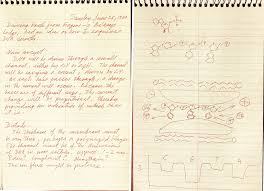
\includegraphics{Nanopore_files/mediabag/9k=.jpg}

}

\caption{Primerio rascunho da ideia da tecnologia de sequênciamento
nanopore}

\end{figure}%

\section{Fluxo de Trabalho}\label{fluxo-de-trabalho}

\begin{verbatim}
Bliblioteca -> sequenciamento -> Análise
\end{verbatim}

\section{Preparo de Biblioteca}\label{preparo-de-biblioteca}

Para o preparo da biblioteca para o sequênciamento de Nanopore é
nescessario adicionar um \texttt{herpin} no fragmento de ssDNA. assim
ligando as duas fitas, possibilitando assim a diferenciação de leitura
da fita
\texttt{5\textquotesingle{}\ -\textgreater{}\ 3\textquotesingle{}} tal
como a fita
\texttt{3\textquotesingle{}\ -\textgreater{}\ 5\textquotesingle{}},
tendo assim uma redundância na leitura e melhorando a precisão.

\subsection{Fragmento de identidicação para
leitura}\label{fragmento-de-identidicauxe7uxe3o-para-leitura}

Esse fragmento de DNA é adicionado a extremidade oposta ao lado com
herpin, e sua função é como calibrador de leitura, e possui
complementariadade a um primer alocado ao poro, assim aumentando a
afinidade e eficiência da leitura. Após este fragmento é adicionado
outro com um \texttt{Barcode}, o qual pode é possível indentidicar
amostras.

\subsection{Adição da DNA
polimerase}\label{adiuxe7uxe3o-da-dna-polimerase}

É necessário adicionar uma enzima que diminua a velocidade de passagem
do DNA do lado \texttt{cis} para o lado \texttt{trans}. E a abertura da
dupla fita a qual possibilida a leitura.

\begin{figure}[H]

{\centering \includegraphics{Nanopore_files/mediabag/Overview-of-the-Nano.png}

}

\caption{Fragmento de DNA pronto na biblioteca}

\end{figure}%

\subsection{Diferenças entre NGS}\label{diferenuxe7as-entre-ngs}

\begin{enumerate}
\def\labelenumi{\arabic{enumi}.}
\tightlist
\item
  equipamento pequeno
\item
  Não precisa amplificar
\end{enumerate}



\end{document}
